\documentclass[12pt letter]{report}
\input{./template/preamble}
\input{./template/macros}
\input{./template/letterfonts}

\title{\Huge{Graphs}}
\author{\huge{Madiba Hudson-Quansah}}
\date{}
\usepackage{parskip}
\usepackage{tikz}
\usepackage{float}

\setcounter{tocdepth}{4}
\setcounter{secnumdepth}{4}

\begin{document}
\maketitle
\newpage
\pdfbookmark[section]{\contentsname}{too}
\tableofcontents
\pagebreak

\chapter{Graphs and Graph Models}

\section{Introduction}

\dfn{Graph}{
  A graph $G = \left( V, E \right) $ consist of $V$, a non empty set of \textit{vertices / nodes} and $E$ a set of
  \textit{edges}. Each edge has either one or two vertices associated with it called its \textit{endpoints}. An edge
  is said to \textit{connect} its endpoints. \\

  The set of vertices $V$ of a graph may be infinite, in this case the graph is called an \textit{infinite graph},
  conversely if the set of vertices is finite, the graph is called a \textit{finite graph}. \\

  The set of edges $E$ contains ordered pairs or sets of elements in the set of vertices $V$ indicating a connection between the
  two nodes or a node to itself.
}

\dfn{Vertex}{
  A \textit{vertex} is a point in a graph. \\
}

\dfn{Edge}{
  An \textit{edge} is a line connecting two vertices in a graph.
}

Below is a graph representing a network of data centres and communication links between computers, where locations are
represented by points and the links are represented by lines connecting the points.

\begin{figure}[H]
  \begin{center}
    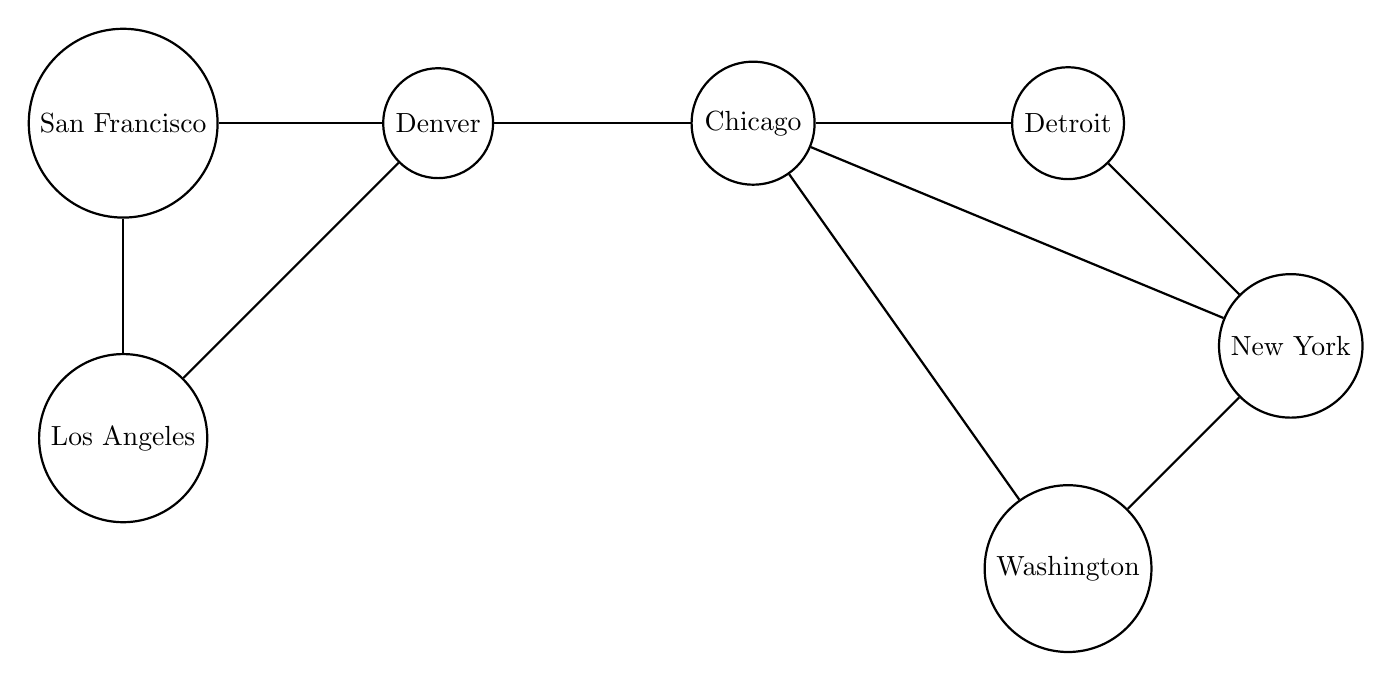
\begin{tikzpicture}[node distance={4cm}, thick, scale=0.5, main/.style = {draw, circle}]
      \node[main] (1) {San Francisco};
      \node[main] (2) [below of=1] {Los Angeles};
      \draw (1) -- (2);
      \node[main] (3) [right of=1] {Denver};
      \draw (1) -- (3);
      \draw (2) -- (3);
      \node[main](4) [right of=3]{Chicago};
      \draw (3) -- (4);
      \node[main] (5) [right of=4] {Detroit};
      \node[main] (6) [below right of=5] {New York};
      \node[main] (7) [below left of=6] {Washington};
      \draw (4) -- (5);
      \draw (4) -- (6);
      \draw (4) -- (7);
      \draw (5) -- (6);
      \draw (6) -- (7);
    \end{tikzpicture}
  \end{center}
  \label{fig:ex1}
\end{figure}

This is an example of a simple graph.

\dfn{Simple Graph}{
  A graph is said to be \textit{simple} if it has no loops or multiple edges. A \textit{loop} is an edge that connects
  a vertex to itself. A \textit{multiple edge} is two or more edges that connect the same pair of vertices. \\
}

\subsection{Multigraph}
This graph could be re-drawn to model multiple links between the same pair of locations, as shown in Figure \ref{fig:ex2}.

\begin{figure}[H]
  \begin{center}
    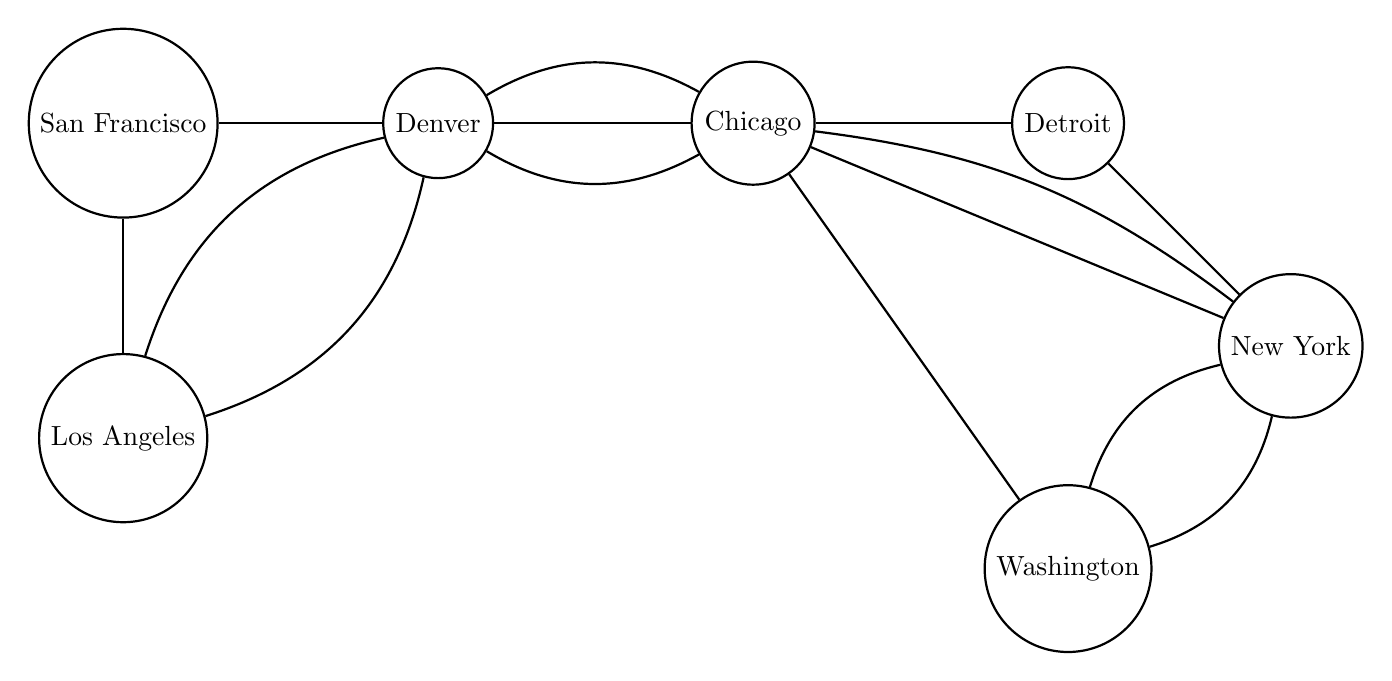
\begin{tikzpicture}[node distance={4cm}, thick, scale=0.5, main/.style = {draw, circle}]
      \node[main] (1) {San Francisco};
      \node[main] (2) [below of=1] {Los Angeles};
      \node[main] (3) [right of=1] {Denver};
      \node[main](4) [right of=3]{Chicago};
      \node[main] (5) [right of=4] {Detroit};
      \node[main] (6) [below right of=5] {New York};
      \node[main] (7) [below left of=6] {Washington};

      \path[every node/.style={font=\sffamily\small}]
      (1) edge (2)
      (1) edge (3)
      (2) edge [bend left] (3)
      (2) edge [bend right] (3)
      (3) edge (4)
      (3) edge [bend right] (4)
      (3) edge [bend left] (4)
      (4) edge (5)
      (4) edge [bend left=15] (6)
      (4) edge (6)
      (5) edge (6)
      (4) edge (7)
      (6) edge[bend right] (7)
      (6) edge[bend left] (7);
    \end{tikzpicture}
  \end{center}
  \label{fig:ex2}
\end{figure}
This is an example of a multigraph.

\dfn{Multigraph}{
  A graph that has multiple edges connecting the same vertices. When there are $m$ distinct edges connecting the same
  unordered pair of vertices $\{u, v\} $, we say that $\{u, v\} $ is an edge of \textit{multiplicity} $m$. i.e. j

}

\subsection{Loops}
Sometimes vertices may be connected to themselves, as shown in Figure \ref{fig:ex3}.
\begin{figure}[H]
  \begin{center}
    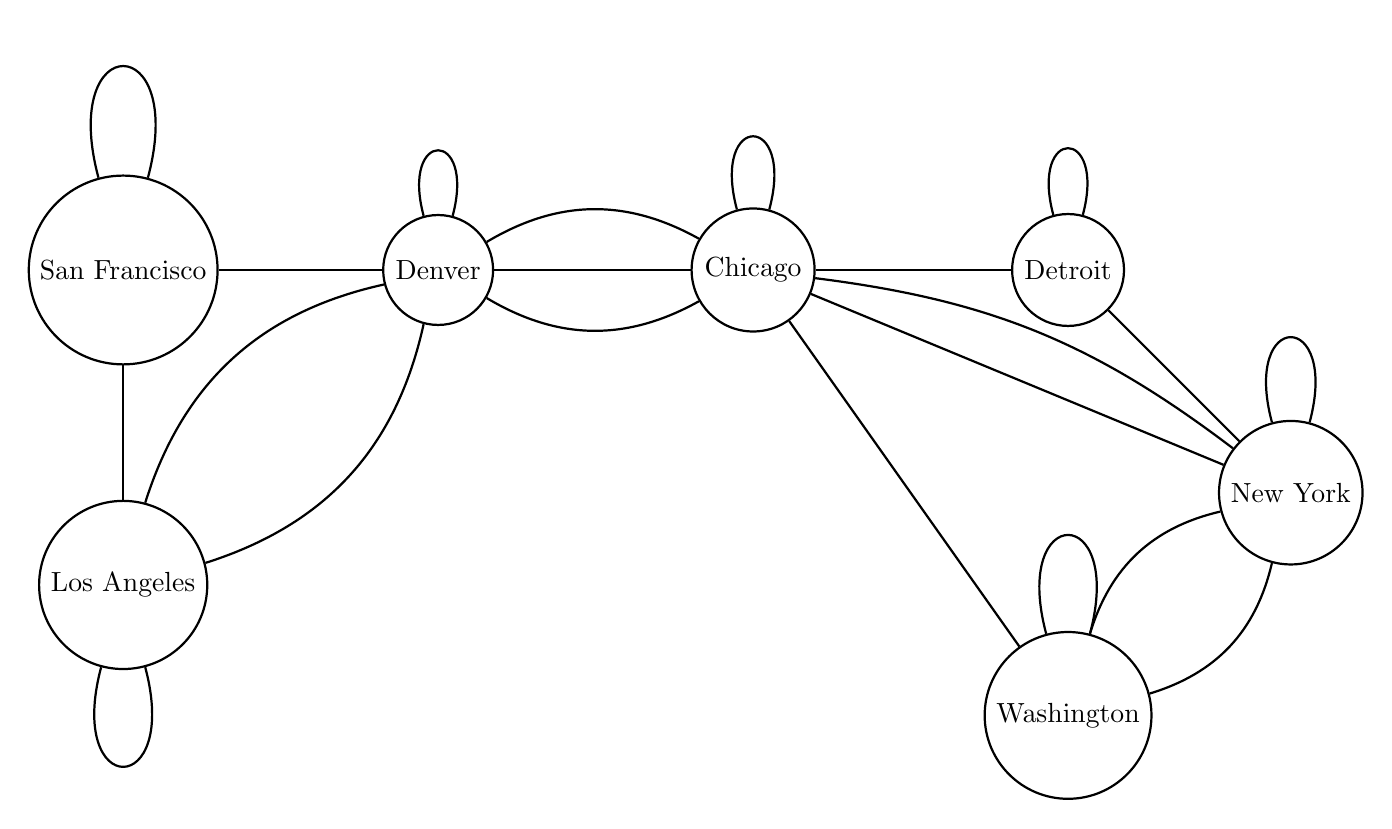
\begin{tikzpicture}[node distance={4cm}, thick, scale=0.5, main/.style = {draw, circle}]
      \tikzset{every loop/.style={}}%removes arrow head from all loops.
      \node[main] (1) {San Francisco};
      \node[main] (2) [below of=1] {Los Angeles};
      \node[main] (3) [right of=1] {Denver};
      \node[main](4) [right of=3]{Chicago};
      \node[main] (5) [right of=4] {Detroit};
      \node[main] (6) [below right of=5] {New York};
      \node[main] (7) [below left of=6] {Washington};

      \path[every node/.style={font=\sffamily\small}]
      (1) edge [loop above] (1)
      (2) edge [loop below] (2)
      (3) edge [loop above] (3)
      (4) edge [loop above] (4)
      (5) edge [loop above] (5)
      (6) edge [loop above] (6)
      (7) edge [loop above] (7)
      (1) edge (2)
      (1) edge (3)
      (2) edge [bend left] (3)
      (2) edge [bend right] (3)
      (3) edge (4)
      (3) edge [bend right] (4)
      (3) edge [bend left] (4)
      (4) edge (5)
      (4) edge [bend left=15] (6)
      (4) edge (6)
      (5) edge (6)
      (4) edge (7)
      (6) edge[bend right] (7)
      (6) edge[bend left] (7);
    \end{tikzpicture}
  \end{center}
  \label{fig:ex3}
\end{figure}

Edges connecting vertices to themselves are called \textit{loops}.
\dfn{Loop}{
  An edge that connects a vertex to itself.
}

\dfn{Psuedograph}{
  A graph that allows loops and multiple edges.

}

\subsection{Directed Graphs}
So far the examples given have been \textit{undirected graphs}, with undirected edges. It is also possible to assign
directions to the edges, as shown in Figure \ref{fig:ex4}.

\begin{figure}[H]
  \begin{center}
    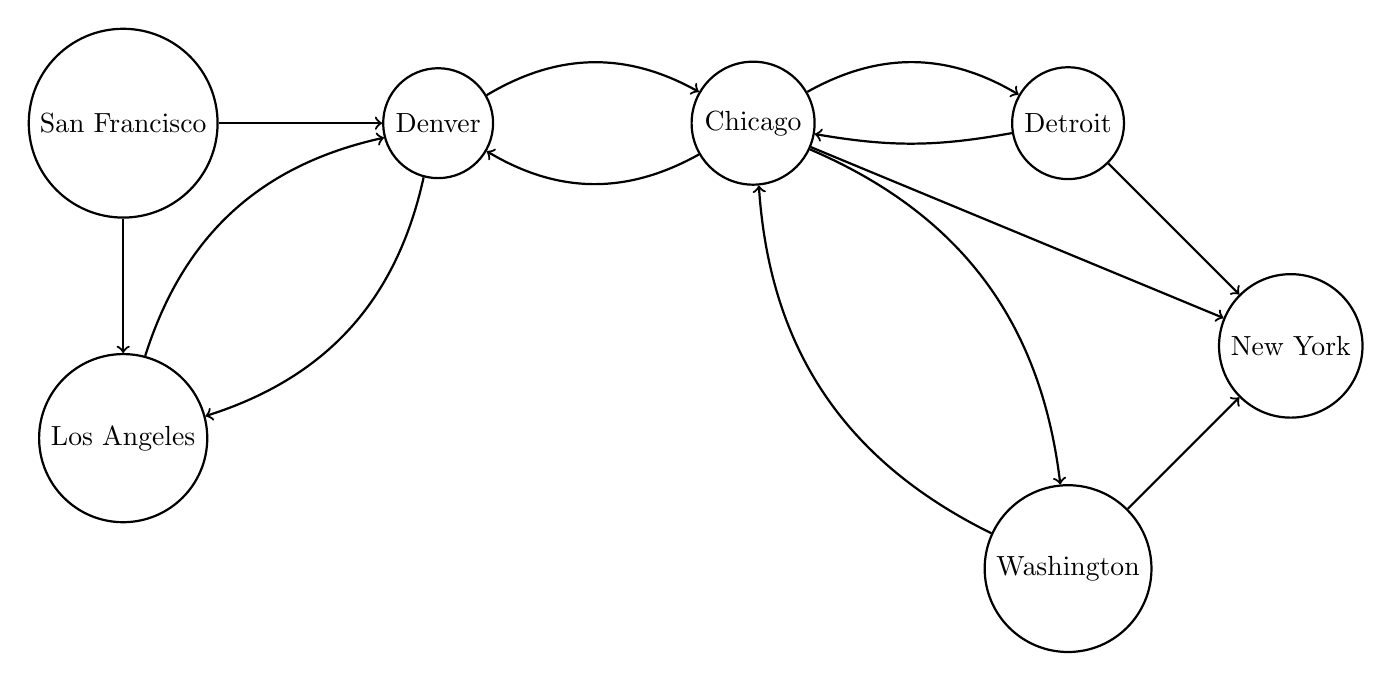
\begin{tikzpicture}[node distance={4cm}, thick, main/.style = {draw, circle}]
      \node[main] (1) {San Francisco};
      \node[main] (2) [below of=1] {Los Angeles};
      \node[main] (3) [right of=1] {Denver};
      \node[main](4) [right of=3]{Chicago};
      \node[main] (5) [right of=4] {Detroit};
      \node[main] (6) [below right of=5] {New York};
      \node[main] (7) [below left of=6] {Washington};

      \path[every node/.style={font=\sffamily\small}]
      (1) edge[->] (2)
      (1) edge[->] (3)
      (2) edge [bend left, ->] (3)
      (2) edge [bend right, <-] (3)
      (3) edge [bend right, <-] (4)
      (3) edge [bend left, ->] (4)
      (4) edge[bend left, ->] (5)
      (4) edge[bend right=10, <-] (5)
      (4) edge[->] (6)
      (5) edge[->] (6)
      (4) edge[bend left, ->] (7)
      (4) edge[bend right, <-] (7)
      (6) edge[<-] (7);
    \end{tikzpicture}
  \end{center}
  \label{fig:ex4}
\end{figure}

Such a graph is called a \textit{directed graph} or \textit{digraph}.

\dfn{Directed Graph}{
  A graph $\left( V, E \right) $ that consists of a non-empty set of vertices $V$ and a set of directed edges / arcs
  $E$. Each directed edge is associated with an ordered pair of vertices. The arc associated with the ordered pair
  $\left( u, v \right) $ is said to \textit{start} at $u$ and \textit{end} at $v$.
}

\subsection{Simple Directed Graph}
\dfn{Simple Directed Graph}{
  A directed graph with no loops or multiple edges.
}

\subsection{Directed Multigraph}
\dfn{Directed Multigraph}{
  A directed graph with multiple edges connecting the same pair of vertices. When there are $m$ directed edges, each
  associated to an ordered pair of vertices $\left( u, v \right) $, then $\left( u, v \right) $ is an edge of
  multiplicity $m$.
}

\subsection{Mixed Graph}
\dfn{Mixed graph}{
  A graph with both direct and undirected edges, that may have multiple edges and loops.
}

\subsection{Graph Terminology}

\begin{table}[htpb]
  \centering
  \begin{tabular}{|c|c|c|c|}
    \hline
    \textit{Type}         & \textit{Edges}          & \textit{Multiple Edges Allowed?} & \textit{Loops Allowed?} \\ [0.5ex]
    \hline
    \hline
    Simple graph          & Undirected              & No                               & No                      \\
    Multigraph            & Undirected              & Yes                              & No                      \\
    Psuedograph           & Undirected              & Yes                              & Yes                     \\
    Simple Directed Graph & Directed                & No                               & No                      \\
    Directed Multigraph   & Directed                & Yes                              & Yes                     \\
    Mixed Graph           & Directed and Undirected & Yes                              & Yes                     \\
    \hline
  \end{tabular}
  \caption{Graph Terminology}
  \label{tab:grp1}
\end{table}

\chapter{Graph Terminology and Special Graphs}

\section{Basic Terminology}

\dfn{Adjacent / Neighbours }{
  Two vertices $u$ and $v$ in an undirected graph $G$, that are endpoints of an edge $e$. Such an edge $e$ is called
  \textit{incident with} the nodes $u$ and $v$ and $e$ is said to \textit{connect} $u$ and $u$
}

\dfn{Neighbourhood}{
  The set of all neighbours of a vertex $v$ of $G = \left( V, E \right) $, denoted by:
  \[
    N \left( v \right)
  \]
  If $A$ is a subset of $V$, we denote by $N \left( A \right) $ the set of all nodes in $G$ that are adjacent to at least one node
  in $A$. i.e. $N \left( A \right) = \bigcup_{v \in A} N \left( v \right)$
}

\dfn{Degree of a Vertex / Node}{
  The number of edges incident with a particular node, except that a loop at a node is counted twice to the degree of
  that node, denoted by:
  \[
    \text{deg}\left( v \right)
  \]
}

\ex{}{
  \qs{}{
    What are the degrees and neighbourhoods of the vertices of the graph below \\

    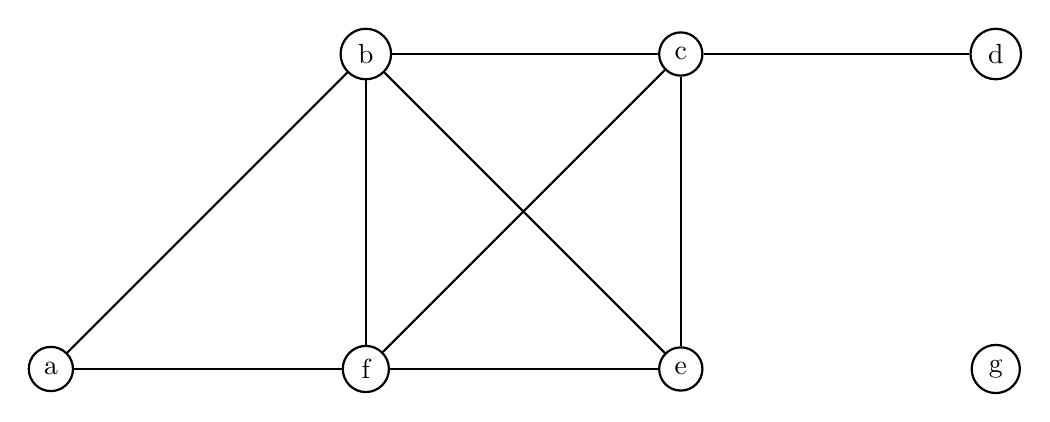
\begin{tikzpicture}[node distance={4cm}, thick, scale=0.5, main/.style = {draw, circle}]
      \node[main] (1) {a};
      \node[main] (2) [right of=1] {f};
      \node[main] (3)[above of=2]{b};
      \node[main](4)[right of=3]{c};
      \node[main](5)[right of=2]{e};
      \node[main](6)[right of=4]{d};
      \node[main](7)[right of=5]{g};
      \path
      (1) edge (2)
      (1) edge (3)
      (3) edge (4)
      (3) edge (5)
      (3) edge (2)
      (2) edge (4)
      (4) edge (5)
      (5) edge (2)
      (4) edge (6)
      ;
    \end{tikzpicture}
  }

  \sol{

    \noindent \underline{Degrees:} \\
    \\
    deg(a) - $2$\\
    deg(b) - $4$\\
    deg(c) - $4$ \\
    deg(d) - $1$\\
    deg(e) - $3$ \\
    deg(f) - $4$ \\
    deg(g) - $0$ \\

    \noindent \underline{Neighbourhoods:}\\
    \\
    \begin{align*}
      N \left( a \right) & = \{b, f\}       \\
      N \left( b \right) & = \{c, f, e, a\} \\
      N \left( c\right)  & = \{b, d, f, e\} \\
      N \left( d \right) & = \{c\}          \\
      N \left( e \right) & = \{b, f, c\}    \\
      N \left( f \right) & = \{b, c, e, a\} \\
      N \left( g \right) & = \O
    \end{align*}
  }
}

\thm{The Handshaking Theorem}{
  Let $G = \left( V, E \right) $ be an undirected graph with $m$ edges. Then
  \[
    2m = \displaystyle\sum_{v \in V} \text{deg}\left( v \right)
  \]
}

\thm{}{
  An undirected graph has an even number of nodes of odd degree.
}

\dfn{Initial and End / Terminal Vertex}{
  When an edge $\left( u, v \right) $, of a directed graph $G$, $u$ is said to be adjacent to $v$ and $v$ is said to be
  adjacent from $u$. $u$ is called the \textit{initial vertex} of $\left( u, v \right) $ and $v$ is called the
  \textit{terminal / end vertex} of $\left( u, v \right) $
}

\dfn{In-degree and Out degree}{
  In a directed graph $G$, the \textit{in-degree} of a vertex $v$, denoted by $\text{deg}^-\left( v \right) $, is the
  number of edges with $v$ as their terminal vertex and the \textit{out-degree} of $v$, denoted by $\text{deg}^+\left( v \right) $,
  is the number of edges with $v$ as their initial vertex.
}

\thm{}{
  Let $G = \left( V, E \right)$ a graph with directed edges. Then
  \[
    \displaystyle\sum_{v \in V}\text{deg}^- \left( v \right)  = \displaystyle\sum_{v \in V}\text{deg}^+ \left( v \right)
    = \,  \mid E \mid
  \]
  Where $ \mid E \mid $ is the number of edges in the graph.
}

\section{Special Graphs}

\subsection{Complete Graphs}

\dfn{Complete Graph}{
  A complete graph $K_n$, on $n$ vertices, is a simple graph that contains exactly one edge between each pair of
  distinct vertices. A simple graph where there it at least one pair of distinct vertices that are not connected by
  a edge is called an \textit{incomplete graph}.
}

\begin{figure}[htpb]
  \centering
  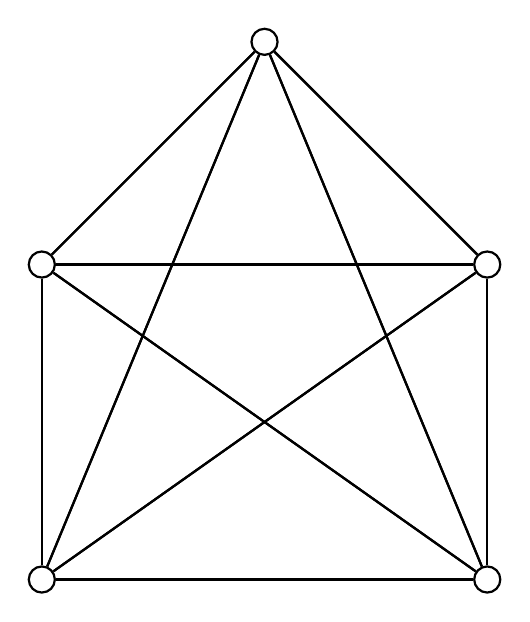
\begin{tikzpicture}[node distance={4cm}, thick, scale=0.5, main/.style = {draw, circle}]
    \node[main] (1) {};
    \node[main] (2)[below right of=1] {};
    \node[main] (3)[below left of=1] {};
    \node[main] (4)[below of=3] {};
    \node[main] (5)[below of=2] {};

    \path
    (1) edge (2)
    (1) edge (3)
    (1) edge (4)
    (1) edge (5)

    (2) edge (1)
    (2) edge (3)
    (2) edge (4)
    (2) edge (5)

    (3) edge (1)
    (3) edge (2)
    (3) edge (4)
    (3) edge (5)

    (4) edge (1)
    (4) edge (2)
    (4) edge (3)
    (4) edge (5)

    (5) edge (1)
    (5) edge (2)
    (5) edge (4)
    (5) edge (3)
    ;
  \end{tikzpicture}
  \caption{$K_5$}
\end{figure}

\subsection{Cycle Graphs}

\dfn{Cycle Graphs}{
  A cycle $C_n$, where $n \geq 3$, consists of $n$ vertices $v_1, v_2, \ldots, v_n$ and edges $\{v_1, v_2\}, \{v_2,
    v_3\} ,\ldots, \{v_{n-1}, \}$ and $\{v_n, v_1\} $.
}

\begin{figure}[htpb]
  \centering
  \begin{tikzpicture}[node distance={4cm}, thick, scale=0.5, main/.style = {draw, circle}]
    \node[main](1){};
    \node[main](2)[below left of=1]{};
    \node[main](3)[below right of=2]{};
    \node[main](4)[right of=1]{};
    \node[main](5)[below right of=4]{};
    \node[main](6)[below left of=5]{};

    \path
    (1) edge (2)
    (2) edge (3)
    (4) edge (5)
    (5) edge (6)
    (3) edge (6)
    (1) edge (4)
    ;
  \end{tikzpicture}
  \caption{$C_6$}
\end{figure}

\subsection{Wheel Graphs}

\dfn{Wheel Graph}{
  A wheel $W_n$ is obtained when an additional vertex is added to a cycle $C_n$, for $n \geq 3$, and connected to each
  of the $n$ vertices of $C_n$, by new edges.
}

\begin{figure}[htpb]
  \centering
  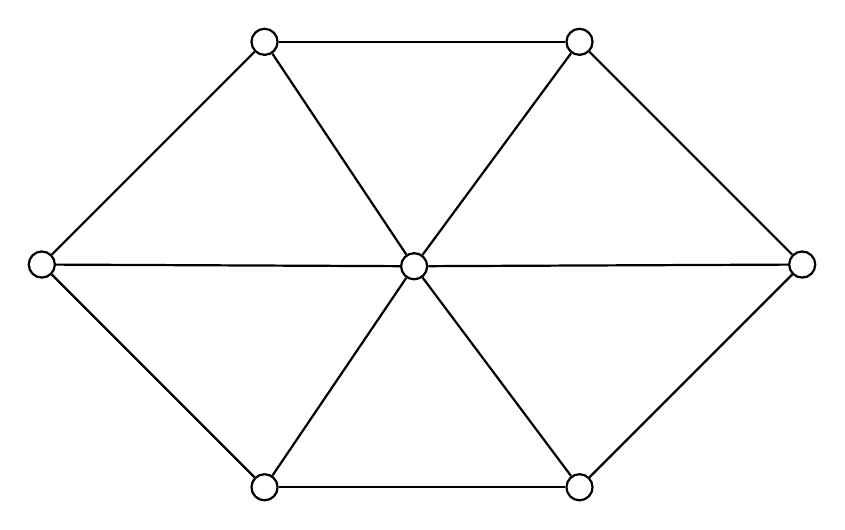
\begin{tikzpicture}[node distance={4cm}, thick, scale=0.5, main/.style = {draw, circle}]
    \node[main](1){};
    \node[main](2)[below left of=1]{};
    \node[main](3)[below right of=2]{};
    \node[main](4)[right of=1]{};
    \node[main](5)[below right of=4]{};
    \node[main](6)[below left of=5]{};

    \node[main] at (3.8, -5.7) (7){};

    \path
    (1) edge (2)
    (2) edge (3)
    (4) edge (5)
    (5) edge (6)
    (3) edge (6)
    (1) edge (4)

    (7) edge (1)
    (7) edge (2)
    (7) edge (3)
    (7) edge (4)
    (7) edge (5)
    (7) edge (6)
    ;
  \end{tikzpicture}
  \caption{$W_6$}
\end{figure}

\section{Bipartite Graphs}

\dfn{Bipartite Graphs}{
  A simple graph $G$ is called \textit{bipartite} if its vertex set $V$ can be partitioned into two disjoint sets $V_1$
  and $V_2$ such that every edge in $G$ connects a vertex in $V_1$ and a vertex in $V_2$, so that no edge in $G$
  connects either two vertices in $V_1$ or two vertices in $V_2$. When this condition holds we call pair $\left( V_1,
    V_2 \right) $ a bipartition of the vertex set $V$ of $G$.
}

\ex{}{
  \qs{}{
    Is the graph below bipartite?\\
    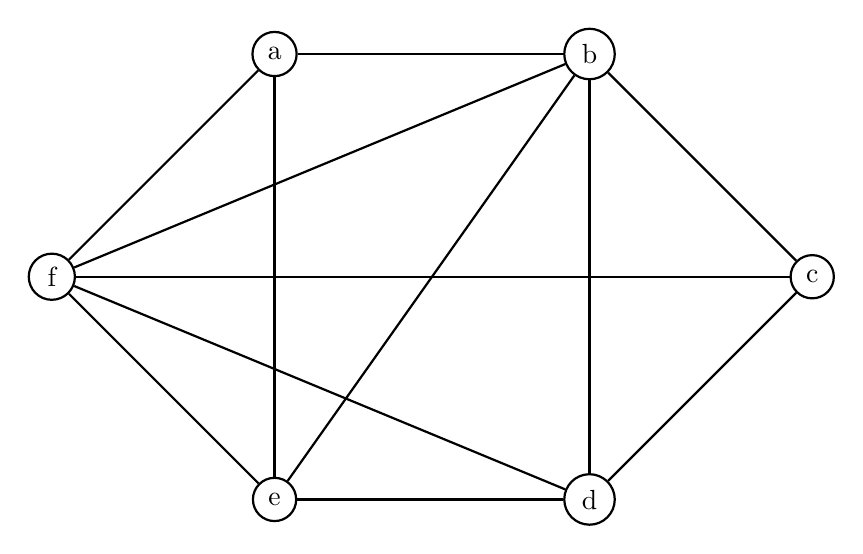
\begin{tikzpicture}[node distance={4cm}, thick, scale=0.5, main/.style = {draw, circle}]
      \node[main](1){a};
      \node[main](2)[below left of=1]{f};
      \node[main](3)[below right of=2]{e};
      \node[main](4)[right of=1]{b};
      \node[main](5)[below right of=4]{c};
      \node[main](6)[below left of=5]{d};

      \path
      (1) edge (2)
      (2) edge (3)
      (4) edge (5)
      (5) edge (6)
      (3) edge (6)
      (1) edge (4)

      (2) edge (4)
      (2) edge (6)
      (2) edge (5)

      (1) edge (3)
      (3) edge (6)
      (3) edge (4)
      (4) edge (6)
      ;
    \end{tikzpicture}
  }

  \sol{
    This graph is not bipartite as there is no vertex set partition which would result in each of elements in set $V_1$
    connecting to at least one element in set $V_2$.
  }
}

\thm{}{
  A simple graph is bipartite if and only  if it is possible to assign one of two different colours to each vertex of
  the graph so that no two adjacent vertices have the same colour.
}

\thm{}{
  A simple graph is bipartite if and only if it is not possible to start a node and return to this node by traversing an odd
  number of distinct edges.
}

\subsection{Complete Bipartite Graphs}

\dfn{Complete Bipartite Graph}{
  A complete bipartite graph $K_{m, n}$ is a bipartite graph with bipartition $\left( m, n \right) $ such that each
  vertex in $m$ is adjacent to every vertex in $n$.
}

\begin{figure}[htpb]
  \centering
  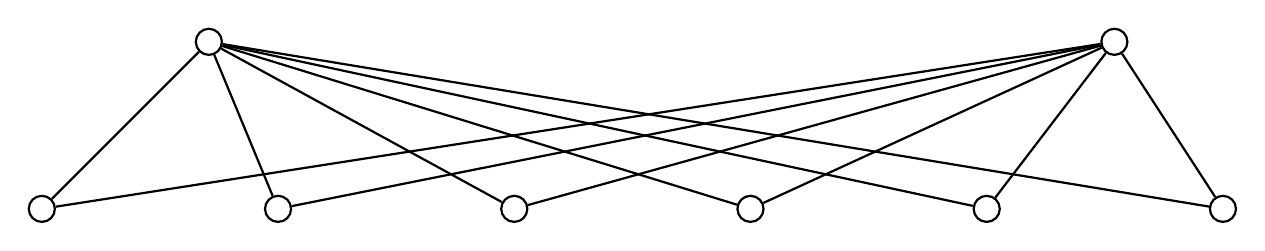
\begin{tikzpicture}[node distance={3cm}, thick, scale=0.5, main/.style = {draw, circle}]
    \node[main] (1) {};
    \node[main] at (23,0) (2) {};

    \node[main] (3)[below left of=1]{};
    \node[main] (4)[right of=3]{};
    \node[main] (5)[right of=4]{};
    \node[main] (6)[right of=5]{};
    \node[main] (7)[right of=6]{};
    \node[main] (8)[right of=7]{};

    \path
    (1) edge (3)
    (1) edge (4)
    (1) edge (5)
    (1) edge (6)
    (1) edge (7)
    (1) edge (8)

    (2) edge (3)
    (2) edge (4)
    (2) edge (5)
    (2) edge (6)
    (2) edge (7)
    (2) edge (8)
    ;
  \end{tikzpicture}
  \caption{$K_{2, 6}$}
\end{figure}

\section{New Graphs From Old}

\subsection{Subgraphs}
\dfn{Subgraph}{
  A \textit{subgraph} of graph $G = \left( V, E \right) $, is a graph $H = \left( W, F \right) $ where $W \subseteq V$
  and $F \subseteq E$. A subgraph $H$ is \textit{proper} if $H \neq G$
}

\dfn{Induced Subgraph}{
  Let $G = \left( V, E \right) $ be a simple graph. The subgraph induced by a subset of $W$ of the node set $V$ is the
  graph $\left( W, F \right) $, where the edge set $F$ contains an edge $E$ if and only if the endpoints of this edge
  are in the node set $W$.
}

Given a graph $G = \left( V, E  \right) $, and an edge $e \in E$, we can produce a subgraph of $G$ by removing $e$ from
the set of edges $E$. The resulting subgraph denoted by $G - e$, has the same node set $V$ as $G$ but with its edge set
$E - e$. Hence:
\[
  G - e = \left( V, E - \{e\}  \right)
\]

Similarly if $E'$ is a subset of $E$, a subgraph of $G$ can be produced by finding the difference of these two sets.
Hence
\[
  G - E' = \left( V, E - E' \right)
\]

We can also add an edge $e$ to a graph to produce a larger graph when this edge connects to two nodes already in $G$,
denoted by $G + e$, where $e$ connects two non-incident nodes in $G$. Hence:
\[
  G + e = \left( V, E \cup \{e\}  \right)
\]
Note that $G + e$ is not a subgraph of $G$.

\dfn{Graph Union}{
  The union of two simple graphs $G_1 = \left( V_1, E_1 \right)  $ and $G_2 = \left( V_2, E_2 \right) $, is the simple
  graph with node set $V_1 \cup V_2$ and edge set $E_1 \cup E_2$, and is denoted:
  \[
    G_1 \cup G_2
  \]
}

\section{Exercises}

\qs{}{
  What do the in-degree and out-degree of a vertex in a web graph represent?
}

\sol{
  The in-degree of a node in a web graph represent the number of pages that link to the node, while the out-degree
  represents the links from the node to other pages.
}

\qs{}{
  What do the in-degree and out-degree of in a directed graph modelling a round-robin tournament represent?
}

\sol{
  In in-degree of a node in this case represents the number of wins that node has had, while the out-degree represents
  the number of losses.
}

\qs{}{
  Show that in a simple graph with at least two vertices, there must be two vertices with the same degree.
}

\sol{
  Using the handshaking theorem, we know that the sum of the degrees of all the vertices in a graph is even. If all the
  vertices in the graph have distinct degrees, then the sum of the degrees of all the vertices in the graph is odd. This
  is a contradiction, hence there must be two vertices with the same degree.
}

\qs{}{
  Draw these graphs:
  \begin{enumerate}
    \item $K_{1,8}$
    \item $W_7$
    \item $C_7$
    \item $Q_4$
  \end{enumerate}
}

\sol{
  \begin{figure}[htpb]
    \centering
    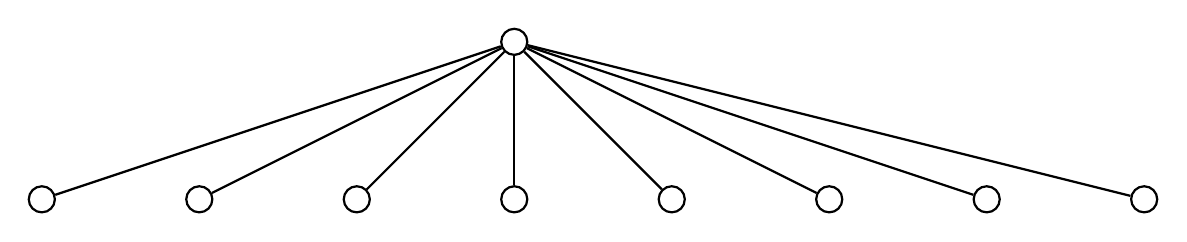
\begin{tikzpicture}[node distance={2cm}, thick, scale=0.5, main/.style = {draw, circle}]
      \node[main](1)[]{};

      \node[main](2) [below of=1]{};

      \node[main](3) [right of=2]{};
      \node[main](4) [right of=3]{};
      \node[main](5) [right of=4]{};
      \node[main](6) [right of=5]{};

      \node[main](7) [left of=2]{};
      \node[main](8) [left of=7]{};
      \node[main](9) [left of=8]{};

      \path
      (1) edge (2)
      (1) edge (3)
      (1) edge (4)
      (1) edge (5)
      (1) edge (6)
      (1) edge (7)
      (1) edge (8)
      (1) edge (9)
      ;
    \end{tikzpicture}
    \caption{$K_{1,8}$}
  \end{figure}

  \begin{figure}[htpb]
    \centering
    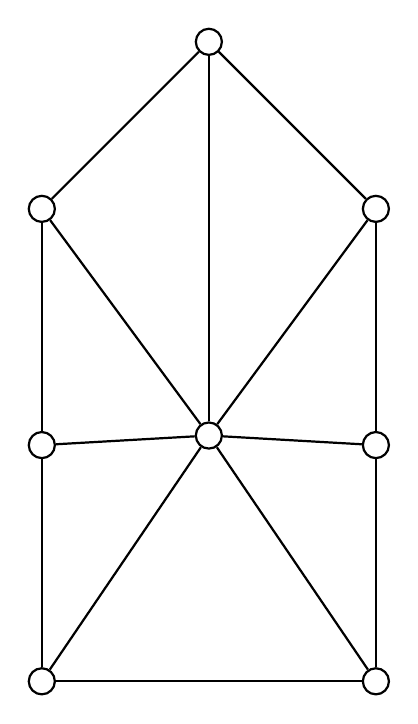
\begin{tikzpicture}[node distance={3cm},thick,main/.style = {draw, circle}]
      \node[main](1){};

      \node[main](2)[below left of=1]{};
      \node[main](3)[below of=2]{};
      \node[main](4)[below  of=3]{};

      \node[main](5)[below right of=1]{};
      \node[main](6)[below of=5]{};
      \node[main](7)[below  of=6]{};

      \node[main] at (0, -5) (8){};

      \path
      (1) edge (2)
      (2) edge (3)
      (3) edge (4)
      (4) edge (7)
      (5) edge (6)
      (6) edge (7)
      (5) edge (1)

      (8) edge (1)
      (8) edge (2)
      (8) edge (3)
      (8) edge (4)
      (8) edge (5)
      (8) edge (6)
      (8) edge (7)
      ;

    \end{tikzpicture}
    \caption{$W_7$}
  \end{figure}

  \begin{figure}[htpb]
    \centering
    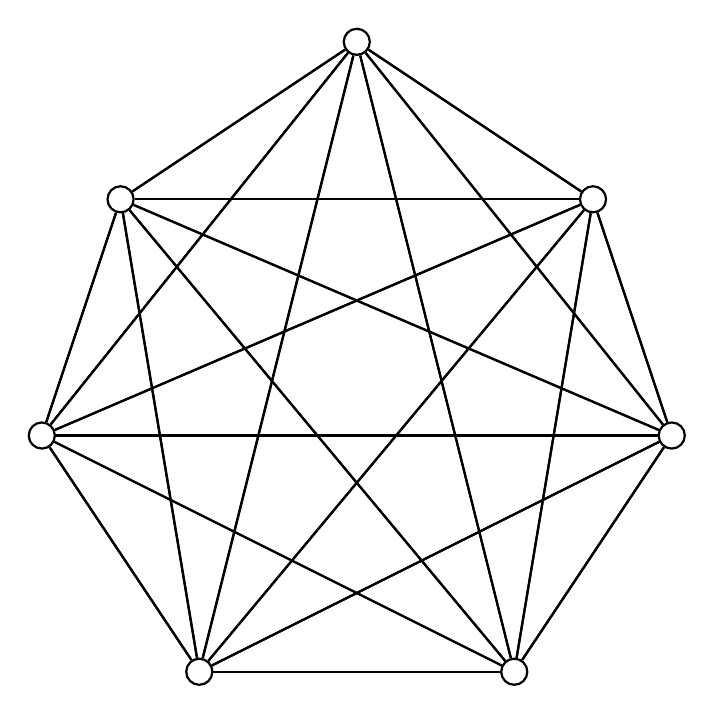
\begin{tikzpicture}[node distance={3cm},thick,main/.style = {draw, circle}]
      \node[main](1){};

      \node[main] at (-3, -2)(2){};
      \node[main] at (-4, -5)(3){};
      \node[main]at (-2, -8)(4){};

      \node[main] at (3, -2) (5){};
      \node[main] at (4, -5)(6){};
      \node[main]at (2, -8)(7){};

      \path
      (1) edge (2)
      (1) edge (3)
      (1) edge (4)
      (1) edge (5)
      (1) edge (6)
      (1) edge (7)

      (2) edge (1)
      (2) edge (3)
      (2) edge (4)
      (2) edge (5)
      (2) edge (6)
      (2) edge (7)

      (3) edge (1)
      (3) edge (2)
      (3) edge (4)
      (3) edge (5)
      (3) edge (6)
      (3) edge (7)

      (4) edge (1)
      (4) edge (2)
      (4) edge (3)
      (4) edge (5)
      (4) edge (6)
      (4) edge (7)

      (5) edge (1)
      (5) edge (2)
      (5) edge (3)
      (5) edge (4)
      (5) edge (6)
      (5) edge (7)

      (6) edge (1)
      (6) edge (2)
      (6) edge (3)
      (6) edge (4)
      (6) edge (5)
      (6) edge (7)

      (7) edge (1)
      (7) edge (2)
      (7) edge (3)
      (7) edge (4)
      (7) edge (5)
      (7) edge (6)
      ;

    \end{tikzpicture}
    \caption{$C_7$}
  \end{figure}
}


\chapter{Representing Graphs and Graph Isomorphism}

\section{Adjacency List}

\dfn{Adjacency List}{
  A list of all the neighbours of each vertex in a graph, showing all the neighbours of each node.
}

\subsection{Simple graph}

\begin{table}[h!]
  \begin{center}
    \begin{tabular}{|c|c|}
      \hline
      Node & Adjacent nodes \\ [0.5ex]
      \hline
      \hline
      $a$  & $b, c, e$      \\
      $b$  & $a$            \\
      $c$  & $a, d, e$      \\
      $d$  & $c, e$         \\
      $e$  & $d, a, c$      \\
      \hline
    \end{tabular}
  \end{center}
\end{table}


\subsection{Directed Graph}

\begin{table}[h!]
  \begin{center}
    \begin{tabular}{|c|c|}
      \hline
      Initial Node & Terminal nodes \\ [0.5ex]
      \hline
      \hline
      $a$          & $b, c,d, e$    \\
      $b$          & $b, d$         \\
      $c$          & $a, c, e$      \\
      $d$          &                \\
      $e$          & $b, c, d$      \\
      \hline
    \end{tabular}
  \end{center}
\end{table}

\section{Adjacency Matrix}

\dfn{Adjacency Matrix}{
  A matrix that represents a graph, either by representing the adjacency of nodes in the graph or the incidences of
  nodes and edges in the graph.
}

\subsection{Adjacency of Nodes}
\subsubsection{Simple Graphs}
\noindent Let $G = \left( V, E \right) $, be a simple graph where $ \mid V \mid  = n$. Suppose that the nodes of $G$ are listed
as $v_1, v_2, \ldots, v_n$. The corresponding adjacency matrix $A$ (or $A_G$) of $G$, with respect to this listing of
nodes is the $n \times n$ zero matrix with $1$ as its $\left( i, j \right) $ entry when $v_i$ and $v_j$ are adjacent,
and $0$ as its $\left( i, j \right) $ entry when they are not adjacent, i.e.:
\begin{align*}
  A      & = \left[ a_{ij} \right]                                \\
  a_{ij} & = \begin{cases}
               1 & \text{if } \{v_i, v_j\} \text{ is an edge of } G \\
               0 & \text{ otherwise}
             \end{cases} \\
\end{align*}
\ex{}{
  \begin{figure}[H]
    \centering
    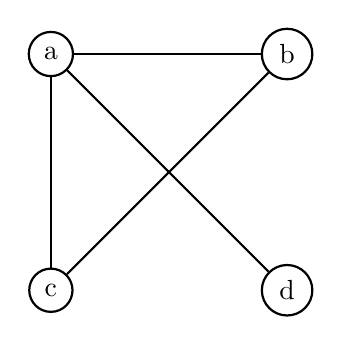
\begin{tikzpicture}[node distance={3cm},thick,main/.style = {draw, circle}]
      \node[main](1){a};
      \node[main](2)[right of=1]{b};
      \node[main](3)[below of=1]{c};
      \node[main](4)[right of=3]{d};

      \path
      (1) edge (2)
      (1) edge (3)
      (1) edge (4)
      (2) edge (3)
      ;

    \end{tikzpicture}
  \end{figure}
  Representing the graph above in an adjacency matrix with nodes listed as $a, b, c, d$:
  \begin{align*}
    \begin{bmatrix}
      0 & 1 & 1 & 1 \\
      1 & 0 & 1 & 0 \\
      1 & 1 & 0 & 0 \\
      1 & 0 & 0 & 0 \\
    \end{bmatrix}
  \end{align*}
}
The adjacency matrix of a simple graph is symmetric, i.e. $a_{ij} = a_{ji}$, because both these entries are $1$ when
$v_i$ or $v_j$ are adjacent. Furthermore, because a simple graph has no loops each entry $a_{ii}$, $i = 1, 2,3,\ldots,
  n$ is $0$.

\subsubsection{Undirected Graphs}
Adjacency matrices can also be used to represent undirected graphs with loops and multiple edges, with loops at the
node $v_i$ represented by a 1 at the $\left( i, i \right) $th position of the matrix, and multiple edges between nodes
$v_i$ and $v_j$ or multiple loops at the same node being represented the number of edges associated with $\{v_i, v_j\} $

\ex{}{
  \begin{figure}[H]
    \centering
    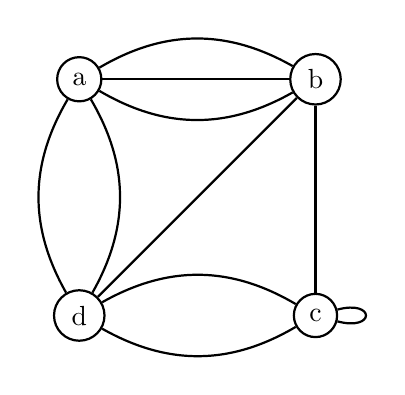
\begin{tikzpicture}[node distance={3cm},thick,main/.style = {draw, circle}]
      \tikzset{every loop/.style={}}%removes arrow head from all loops.
      \node[main](1){a};
      \node[main](2)[right of=1]{b};
      \node[main](3)[below of=1]{d};
      \node[main](4)[right of=3]{c};

      \path[every node/.style={font=\sffamily\small}]
      (1) edge (2)
      (1) edge[bend right] (2)
      (1) edge[bend left] (2)
      (1) edge[bend right](3)
      (1) edge[bend left](3)

      (2) edge (3)
      (2) edge (4)

      (3) edge[bend right](4)
      (3) edge[bend left](4)
      (4) edge [loop right](4)
      ;

    \end{tikzpicture}
  \end{figure}
  Representing the graph above with an adjacency matrix with nodes listed as $a, b, c, d$:
  \begin{align*}
    \begin{bmatrix}
      0 & 3 & 0 & 2 \\
      3 & 0 & 1 & 1 \\
      0 & 1 & 1 & 2 \\
      2 & 1 & 2 & 0 \\
    \end{bmatrix}
  \end{align*}
}

\subsubsection{Directed Graphs}

The matrix for a directed graph $G = \left( V, E \right) $ has a $1$ in its $\left( i, j \right) $th position if there
is an edge from $v_i$ to $v_j$, where $v_1, v_2, \ldots, v_n$ is an arbitrary listing of the nodes of the graph.
Therefore:
\begin{align*}
  A      & = \left[ aij \right]                                              \\
  a_{ij} & = \begin{cases}
               1 & \text{if } \left( v_i, v_j \right) \text{ is an edge of } G \\
               0 & \text{ otherwise}
             \end{cases}
\end{align*}

\subsection{Incidence of Nodes and Edges / Incidence Matrix}

\dfn{Incidence Matrix}{
  Let $G  = \left( V, E \right) $, be an undirected graph, with an arbitrary listing of nodes $v_1, v_2, \ldots, v_n$
  and edges $e_1, e_2, \ldots, e_m$. The incidence matrix with respect to this listing of nodes and edges is the $n
    \times m$ matrix:
  \begin{align*}
    m_{ij} = \begin{cases}
               1 & \text{ when edge } e_j \text{ is incident with node } v_i \\
               0 & \text{ otherwise}
             \end{cases}
  \end{align*}
}

\ex{}{
  \begin{figure}[H]
    \centering
    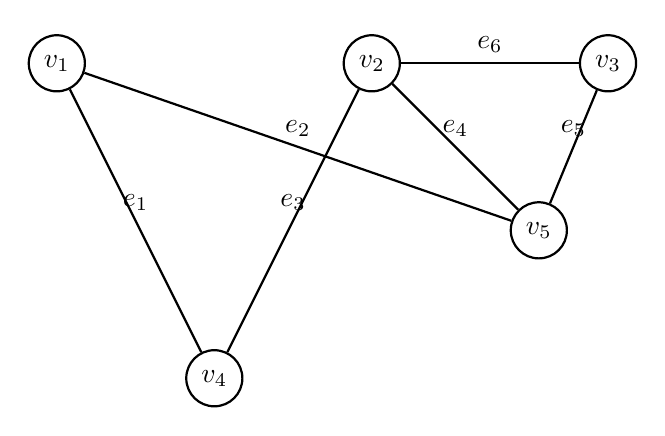
\begin{tikzpicture}[node distance={3cm},thick,main/.style = {draw, circle}]
      \node[main](1){$v_1$};
      \node[main]at (4, 0)(2){$v_2$};
      \node[main](3)[right of=2]{$v_3$};
      \node[main]at (2, -4) (4){$v_4$};
      \node[main](5)[below right of=2]{$v_5$};

      \path
      (1) edge node[above]{$e_1$} (4)
      (1) edge node[above]{$e_2$} (5)

      (4) edge node[above]{$e_3$}(2)
      (2) edge node[above]{$e_4$}(5)
      (5) edge node[above]{$e_5$}(3)
      (2) edge node[above]{$e_6$}(3)
      ;
    \end{tikzpicture}
  \end{figure}
  Representing the graph above with an incidence matrix with the already listed order of nodes and edges:
  \begin{align*}
    M =   \begin{bmatrix}
            1 & 1 & 0 & 0 & 0 & 0 \\
            0 & 0 & 1 & 1 & 0 & 1 \\
            0 & 0 & 0 & 0 & 1 & 1 \\
            1 & 0 & 1 & 0 & 0 & 0 \\
            0 & 1 & 0 & 1 & 1 & 0 \\
          \end{bmatrix}
  \end{align*}
}

Incidence matrices can also be used to represent multiple edges and loops, with multiple edges represented in the matrix
using columns with identical entries as these edges are incident with the same pair of nodes, and loops represented as a
column with exactly one entry equal to $1$, corresponding to the node that is incident with the loop.

\section{Isomorphism of Graphs}

\dfn{Isomorphic Graphs}{
  Two simple graphs $G_1 = \left( V_1, E_1 \right) $ and $G_2 = \left( V_2, E_2 \right) $ are \textit{isomorphic} if
  there exists a one-to-one and onto function $f$ from $V_1$ to $v_2$ with the property that $a$ and $b$ are adjacent in
  $G_1$ if and only if $f \left( a \right) $ and $f \left( b \right) $ are adjacent in $G_2$, for all $a$ and $b$ in
  $V_1$. This function $f$ is called an \textit{isomorphism}, and two graphs that are not isomorphic are called
  \textit{nonisomorphic}.
}

\ex{}{
  \qs{}{
    Show that the graphs $G = \left( V, E \right) $ and $H = \left( W, F \right) $ below are isomorphic:
    \begin{figure}[H]
      \centering
      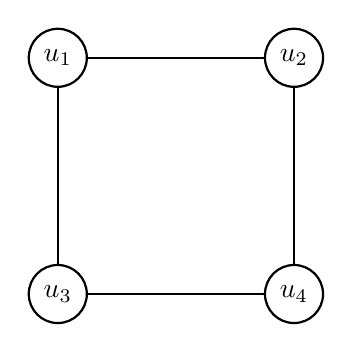
\begin{tikzpicture}[node distance={3cm},thick,main/.style = {draw, circle}]
        \node[main](1){$u_1$};
        \node[main](2)[right of=1]{$u_2$};
        \node[main](3)[below of=1]{$u_3$};
        \node[main](4)[below of=2]{$u_4$};

        \path
        (1) edge (2)
        (2) edge (4)
        (3) edge (4)
        (1) edge (3)
        ;
      \end{tikzpicture}
      \caption{$G$}
    \end{figure}
    \begin{figure}[H]
      \centering
      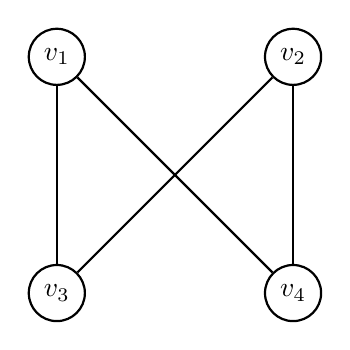
\begin{tikzpicture}[node distance={3cm},thick,main/.style = {draw, circle}]
        \node[main](1){$v_1$};
        \node[main](2)[right of=1]{$v_2$};
        \node[main](3)[below of=1]{$v_3$};
        \node[main](4)[below of=2]{$v_4$};

        \path
        (1) edge (3)
        (2) edge (4)
        (1) edge (4)
        (3) edge (2)
        ;
      \end{tikzpicture}
      \caption{$H$}
    \end{figure}
  }

  \sol{

    The function $f$ with $f \left( u_1 \right) = v_1, f \left( u_2 \right) = v_4, f \left( u_3 \right) = v_3, f \left(
      u_4\right) = v_2   $ is a one-to-one correspondence between $V$ and $W$. With the correspondence preserving
    adjacency as all the adjacent pairs in graph $G$, $\{u_1, u_2\} $, $\{u_2, u_4\} $, $\{u_3, u_4\} $, $\{u_3, u_4\}
    $, are preserved in the graph $H$ as $\{v_1, v_4\} $, $\{v_1, v_3\} $, $\{v_3, v_2\} $, $\{v_2, v_4\} $
  }
}

\subsection{Determining Isomorphism of Two Simple Graphs}

It is difficult to determine the isomorphism of two simple graphs as there are $n!$ possible one-to-one correspondences
between the nodes of the two graphs with $n$ nodes. However sometimes  it is not hard to show that two graphs are
nonisomorphic. We can do this by finding one property only one of the two graphs has, but that is preserved by
isomorphism, this is called a graph \textit{invariant}.

\dfn{Graph Invariant}{
  A property of one graph that is preserved by isomorphism, and that is not shared by another graph. For example the
  number of nodes in a graph is a graph invariant.
}

Two graphs cannot be isomorphic if they do not have the following properties:
\begin{itemize}
  \item The same number of nodes as there must be a one-to-one correspondence between the nodes of the two graphs.
  \item The same number of edges as the one-to-one correspondence between node preserves the one-to-one correspondence
        between edges.
  \item The same degrees for each node correspondence between each graph.
\end{itemize}

\chapter{Exercises}

\qs{}{
  Draw $K_5$ and $\overline{K_5}$
}

\sol{

  $K_5$: \\
  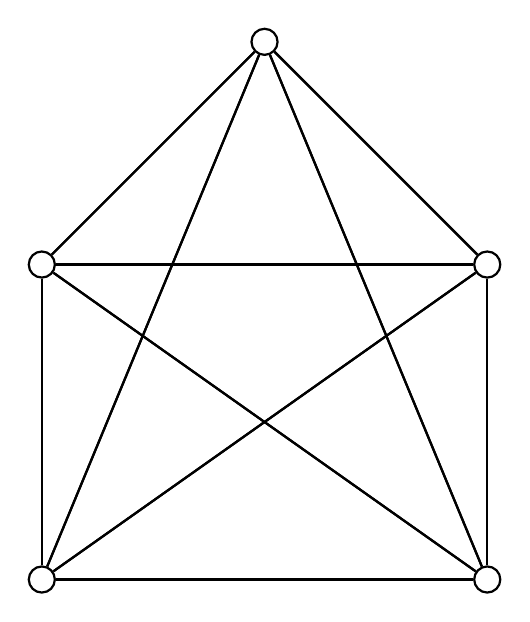
\begin{tikzpicture}[node distance={4cm}, thick, scale=0.5, main/.style = {draw, circle}]
    \node[main] (1) {};
    \node[main] (2)[below right of=1] {};
    \node[main] (3)[below left of=1] {};
    \node[main] (4)[below of=3] {};
    \node[main] (5)[below of=2] {};

    \path
    (1) edge (2)
    (1) edge (3)
    (1) edge (4)
    (1) edge (5)

    (2) edge (1)
    (2) edge (3)
    (2) edge (4)
    (2) edge (5)

    (3) edge (1)
    (3) edge (2)
    (3) edge (4)
    (3) edge (5)

    (4) edge (1)
    (4) edge (2)
    (4) edge (3)
    (4) edge (5)

    (5) edge (1)
    (5) edge (2)
    (5) edge (4)
    (5) edge (3)
    ;
  \end{tikzpicture}
  \\

  $\overline{K_5}$:\\
  \begin{tikzpicture}[node distance={4cm}, thick, scale=0.5, main/.style = {draw, circle}]
    \node[main] (1) {};
    \node[main] (2)[below right of=1] {};
    \node[main] (3)[below left of=1] {};
    \node[main] (4)[below of=3] {};
    \node[main] (5)[below of=2] {};
  \end{tikzpicture}

}

\end{document}
